% F3 — CI/CD pipeline (swimlane diagram)
% Standalone TikZ figure: compile with lualatex or pdflatex.
% The enclosing chapter supplies \caption{}; no caption text lives here.
\documentclass[tikz,border=8pt]{standalone}
\usetikzlibrary{positioning, arrows.meta, shapes.geometric, backgrounds, fit, calc}

\begin{document}
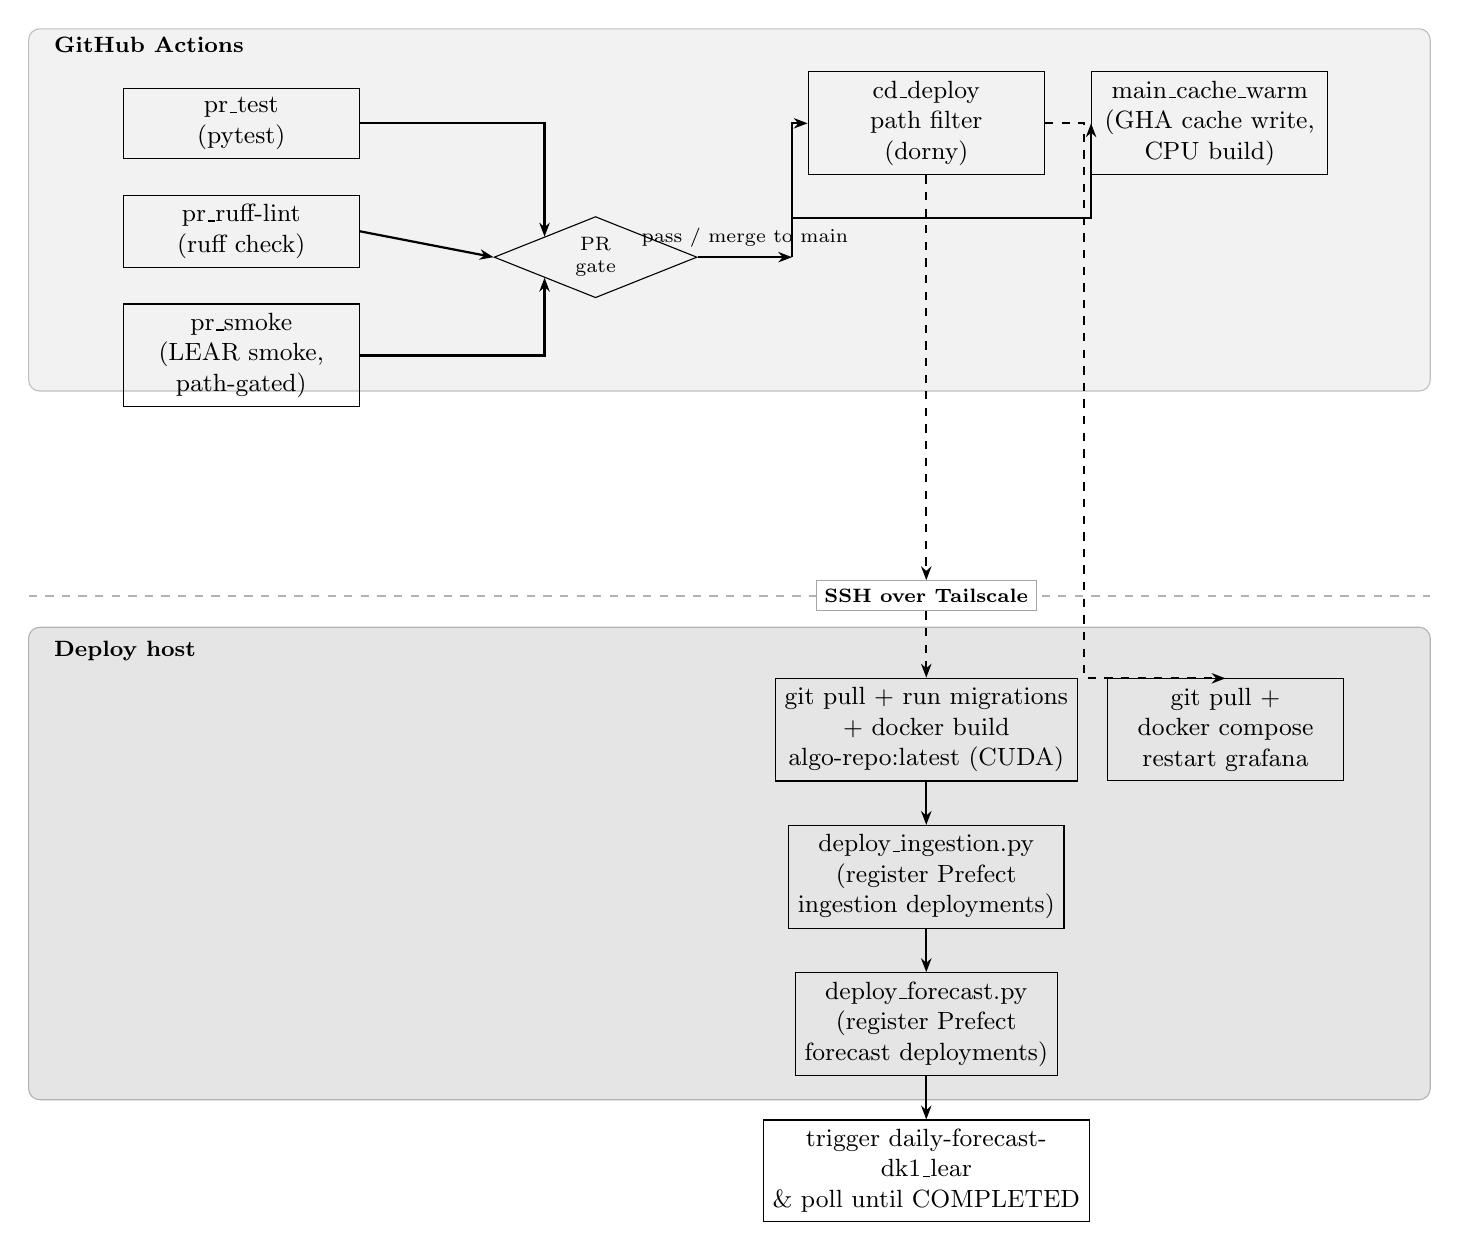
\begin{tikzpicture}[
  % --- node styles ---
  pipestep/.style={
    draw, rectangle,
    minimum width=3.0cm, minimum height=0.85cm,
    align=center, font=\small
  },
  gate/.style={
    draw, diamond,
    minimum width=2.2cm, minimum height=0.85cm,
    align=center, font=\scriptsize,
    aspect=2.5
  },
  lane_label/.style={
    font=\footnotesize\bfseries, anchor=west
  },
  % --- arrow styles ---
  arr/.style={-{Stealth[length=5pt]}, thick},
  darr/.style={-{Stealth[length=5pt]}, thick, dashed},
]

% -------------------------------------------------------
% LANE LAYOUT (fixed coordinates)
%   GitHub Actions lane  :  y in [2.8, 7.4]
%   Lane separator       :  y = 0.2
%   Deploy host lane     :  y in [-6.2, -0.2]
% -------------------------------------------------------

% ============================================================
% GITHUB ACTIONS LANE
% ============================================================

% --- PR-time workflows (left cluster, stacked vertically) ---
\node[pipestep] (pr_test)
    at (-7.5, 6.2)
    {pr\_test\\(pytest)};

\node[pipestep] (pr_lint)
    [below=0.45cm of pr_test]
    {pr\_ruff-lint\\(ruff check)};

\node[pipestep] (pr_smoke)
    [below=0.45cm of pr_lint]
    {pr\_smoke\\(LEAR smoke,\\path-gated)};

% PR gate diamond (centre of lane, horizontally between PR jobs and post-merge)
\node[gate] (pr_gate)
    at (-3.0, 4.5)
    {PR\\gate};

% --- Post-merge (push to main) workflows ---
\node[pipestep] (cd_changes)
    at (1.2, 6.2)
    {cd\_deploy\\path filter\\(dorny)};

\node[pipestep] (cache_warm)
    at (4.8, 6.2)
    {main\_cache\_warm\\(GHA cache write,\\CPU build)};

% ============================================================
% DEPLOY HOST LANE
% ============================================================

\node[pipestep] (build_img)
    at (1.2, -1.5)
    {git pull + run migrations\\+ docker build\\algo-repo:latest (CUDA)};

\node[pipestep] (deploy_ing)
    [below=0.55cm of build_img]
    {deploy\_ingestion.py\\(register Prefect\\ingestion deployments)};

\node[pipestep] (deploy_fcast)
    [below=0.55cm of deploy_ing]
    {deploy\_forecast.py\\(register Prefect\\forecast deployments)};

\node[pipestep] (reload_gf)
    at (5.0, -1.5)
    {git pull +\\docker compose\\restart grafana};

\node[pipestep] (smoke_run)
    [below=0.55cm of deploy_fcast]
    {trigger daily-forecast-\\dk1\_lear\\\& poll until COMPLETED};

% ============================================================
% ARROWS — GitHub Actions lane
% ============================================================

% PR workflows → gate
\draw[arr] (pr_test.east)  -| (pr_gate.north west);
\draw[arr] (pr_lint.east)  -- (pr_gate.west);
\draw[arr] (pr_smoke.east) -| (pr_gate.south west);

% Gate → intermediate merge point, then fan out to post-merge workflows
\coordinate (merge_pt) at ($(pr_gate.east)+(1.2,0)$);

\draw[arr] (pr_gate.east) -- (merge_pt)
    node[midway, above, font=\scriptsize] {pass / merge to main};

\draw[arr] (merge_pt) |- (cd_changes.west);
\draw[arr] (merge_pt) -- ++(0,0.5) -| (cache_warm.west);

% ============================================================
% SSH OVER TAILSCALE boundary label (sits on lane separator)
% ============================================================

\node[draw=gray!70, rectangle, fill=white, inner sep=3pt,
      font=\scriptsize\bfseries]
    (ssh_label)
    at (1.2, 0.2)
    {SSH over Tailscale};

% ============================================================
% ARROWS — GitHub Actions → Deploy host (cross-lane, dashed)
% ============================================================

% cd_changes → build_img (via SSH; path: image or shared)
\draw[darr] (cd_changes.south) -- ++(0,-0.6) -| (ssh_label.north);
\draw[darr] (ssh_label.south) -- (build_img.north);

% cd_changes → reload_grafana (via SSH; path: grafana)
\draw[darr] (cd_changes.east) -- ++(0.5,0) |- (reload_gf.north);

% ============================================================
% ARROWS — Deploy host internal (solid)
% ============================================================

\draw[arr] (build_img.south)   -- (deploy_ing.north);
\draw[arr] (deploy_ing.south)  -- (deploy_fcast.north);
\draw[arr] (deploy_fcast.south) -- (smoke_run.north);

% ============================================================
% SWIMLANE BACKGROUNDS (drawn behind all nodes)
% ============================================================

\begin{pgfonlayer}{background}
  % GitHub Actions lane
  \fill[gray!10, draw=gray!50, rounded corners=4pt]
      (-10.2, 2.8) rectangle (7.6, 7.4);

  % Deploy host lane
  \fill[gray!20, draw=gray!60, rounded corners=4pt]
      (-10.2, -6.2) rectangle (7.6, -0.2);

  % Lane separator
  \draw[gray!60, dashed, line width=0.7pt]
      (-10.2, 0.2) -- (7.6, 0.2);
\end{pgfonlayer}

% ============================================================
% LANE LABELS
% ============================================================

\node[lane_label] at (-10.0, 7.2)  {GitHub Actions};
\node[lane_label] at (-10.0, -0.5) {Deploy host};

\end{tikzpicture}
\end{document}
